\section{Numeric Abstraction}
\label{sec:numeric-abstraction}

\begin{figure}[hb]
    \centering
    \begin{tikzpicture}[auto,node distance=18mm]
    \node[rectangle, minimum size=7mm, draw, fill, red]  (r1) {};
    \node[rectangle, minimum size=7mm, draw, fill, blue] (b1) [below left of=r1] {};
    \node[rectangle, minimum size=7mm, draw, fill, blue] (b2) [below right of=r1] {};
    \node[rectangle, minimum size=7mm, draw, fill, red]  (r2) [below left of=b2] {};
    \node[rectangle, minimum size=7mm, draw, fill, blue] (b3) [right of=r2] {};
    \node[rectangle, minimum size=7mm, draw, fill, red]  (r3) [right of=b3] {};

    \node[shape=diamond, draw, fill, black]  (t1) at (b1.center) {};
    \node[shape=diamond, draw, fill, black]  (t2) at (b2.center) {};
    \node[shape=diamond, draw, fill, black]  (t3) at (b3.center) {};

    \path (r1) edge (b1)
          (r1) edge (b2)
          (b1) edge (r2)
          (b2) edge (r2)
          (r2) edge (b3)
          (b3) edge (r3);
  \end{tikzpicture}
  \qquad
  \begin{tikzpicture}[auto,node distance=18mm]
    \node[rectangle, minimum size=7mm, draw, fill, red]  (r1) {};
    \node[rectangle, minimum size=7mm, draw, fill, blue] (b1) [below left of=r1] {};
    \node[rectangle, minimum size=7mm, draw, fill, blue] (b2) [below right of=r1] {};
    \node[rectangle, minimum size=7mm, draw, fill, red]  (r2) [below left of=b2] {};
    \node[rectangle, minimum size=7mm, draw, fill, blue] (b3) [right of=r2] {};
    \node[rectangle, minimum size=7mm, draw, fill, red]  (r3) [right of=b3] {};

    \node[shape=diamond, draw, fill, black]  (t1) at (r1.center) {};
    \node[shape=diamond, draw, fill, black]  (t2) at (r2.center) {};
    \node[shape=diamond, draw, fill, black]  (t3) at (r3.center) {};

    \path (r1) edge (b1)
          (r1) edge (b2)
          (b1) edge (r2)
          (b2) edge (r2)
          (r2) edge (b3)
          (b3) edge (r3);
  \end{tikzpicture}

  \bigskip
  \bigskip
  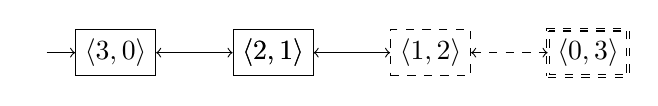
\begin{tikzpicture}[auto,node distance=2cm]
    \node (init) at (0, 0) {};
    \node[draw] (n30) at (1, 0) {$\langle 3,0 \rangle$};
    \node[draw] (n21) [right of=n30] {$\langle 2,1 \rangle$};
    \node[draw] (n21) [right of=n30] {$\langle 2,1 \rangle$};
    \node[draw,dashed] (n12) [right of=n21] {$\langle 1,2 \rangle$};
    \node[draw,dashed,double] (n03) [right of=n12] {$\langle 0,3 \rangle$};

    \path[draw,->] (init) edge (n30);
    \path[draw,<->] (n30) edge (n21);
    \path[draw,<->] (n21) edge (n12);
    \path[draw,<->,dashed] (n12) edge (n03);
  \end{tikzpicture}
  \caption{ Example coloring for numeric abstraction. The initial state is on
      the left and the goal state on the right. Nodes are colored blue if they have a
      token in the initial state but not the goal state and red if they have no token
      in the initial state but a token in the goal state. The abstract state space is
      shown below the instance. Dashed nodes are pruned.}
  \label{fig:numeric-abstractions-example}
\end{figure}

The \emph{numeric abstraction} component of our solver tries to detect if the
task is unsolvable by abstracting it to a numeric planning problem. Given an ISR
problem, we come up with a \emph{coloring} of the vertices in the graph, i.e., a
function that maps each vertex of the graph to one color. Many different ways of
coming up with a good coloring are conceivable but here we opted for a simple
strategy that uses up to four colors:
\begin{itemize}
    \item one for nodes that contain a token both in the initial state and in the goal state;
    \item one for nodes that contain a token only in the initial state but not in the goal state;
    \item one for nodes that contain a token only in the goal state but not in the initial state; and
    \item one for nodes that are empty in the initial state and goal state.
\end{itemize}

Colors for situations that do not occur are not used. For example, the task in
Figure~\ref{fig:numeric-abstractions-example} only requires two colors with the
method above.

Given a coloring, each configuration of tokens can be abstracted to a state with
one numeric variable per color that counts how many token currently are on
vertices with this color. For example, the initial state in
Figure~\ref{fig:numeric-abstractions-example} has 3 tokens on blue nodes and 0
on red nodes, so it can be represented as the numeric state $\langle 3,
0\rangle$. The goal state has all three tokens on red nodes and none on blue, so
it can represented by $\langle 0, 3 \rangle$.

Moving any token from a node colored $c_i$ to a node colored $c_j$ changes the
abstract state from $\langle c_1, \dots, c_i, \dots, c_j, \dots, c_n \rangle$ to
$\langle c_1, \dots, c_i-1, \dots, c_j+1, \dots, c_n \rangle$. The main
observation for this component is that if any solution to the full problem
exists, there has to be a solution in our abstraction as well. We thus construct
the state space of the abstraction in the following way.

For a state $s = \langle c_1, \dots, c_n \rangle$, we construct one successor
for each pair of different colors $c_i$ and $c_j$ that differs from $s$ by a
single token that moved from $c_i$ to $c_j$. In our running example, the initial
state $\langle 3, 0\rangle$ has a single successor $\langle 2, 1\rangle$, and
this state has two successors $\langle 3, 0\rangle$ (which we skip because we
have already seen this state) and $\langle 1, 2\rangle$. The latter state now
has the abstract goal state $\langle 0, 3\rangle$ as a successor (see
Figure~\ref{fig:numeric-abstractions-example}).

Whenever we generate a state, we check whether such a state is possible
(independent of whether we are actually able to reach such a state). If it is
not possible to place the token on the respective colors in the way suggest,
then we do not have to consider it or its successors. In our running example,
the state $\langle 1, 2 \rangle$ is not realizable: not matter where we place
the blue token, it blocks two of the three red nodes. We use a MIP solver to
check if a state $s$ is realizable by checking if the following system of
constraints have a solution:

\begin{align*}
    x_i + x_j &\le 1 \quad \text{for all edges $\langle i, j \rangle$ in the graph}\\
    \sum_{i \in N_c} x_i &\ge s[c] \quad \text{for all colors $c$} \\
    x_i \in \{0, 1\} & \qquad\text{for all nodes $i$}
\end{align*}
where $N_c$ is a set of all nodes with color $c$ and $s[c]$ is the amount of
tokens that should be on color $c$ in state $s$. The abstract state $s$ is realizable iff the
constraints have a solution.

If we generate a state that matches the goal state ($\langle 0, 3\rangle$ in our
example), we know that there is an abstract path to the goal state. In this case, we
still do not know if there is a real path to the goal state and return
\texttt{unknown} (this component of the solver is incomplete). However, if we
expand the full abstract state space without finding a path to an abstract goal
state, there is no solution to the abstract problem which also means there
cannot be a solution to the original problem. The abstract state space is
usually small. In our running example, it only has 4 states and we only have to
explore 3 of them, as we prune state $\langle 1, 2 \rangle$ before reaching a
goal state.

We use this component in two places: first with a small time limit at the start of
the solver to handle all cases where we can quickly prove unsolvability. Then
again with a large time limit after all other components to catch unsolvable
instances that are hard to prove unsolvable.
